
\section{Hello World Example\marginnote{(Demonstration of Basic UxAS configuration and service to service communication)}}
This is an introductory example to UxAS. The UxAS service \textbf{\textit{HelloWorld}} is designed to perodically send and receive \textit{KeyValuePair} messages. Parameters for the service are \textit{StringToSend} and \textit{SendPeriod\_ms}. As the names imply, \textit{StringToSend} is the string sent from the service and \textit{SendPeriod\_ms} is how often, in milliseconds, the string will be sent. Each instance of the \textbf{\textit{HelloWorld}} service subscribes to \textit{KeyValuePair} messages, which means that it will receive any of these messages sent from other services. The configuration file for this example,
\begin{docspec}
\textit{uxas/examples/01\_HelloWorld/cfg\_HelloWorld.xml}
\end{docspec}
contains entries for two instances of \textbf{\textit{HelloWorld}}:

\begin{fullwidth}
\begin{docspec}
    <Service Type="HelloWorld" StringToSend="Hello from \#1" SendPeriod\_ms="1000"/>
\end{docspec}
\begin{docspec}
    <Service Type="HelloWorld" StringToSend="Hello from \#2" SendPeriod\_ms="5001"/>
\end{docspec}
\end{fullwidth}

As the example runs, both instances send \textit{KeyValuePair} messages and each instance receives these messages from the other. Figure \ref{fig:HelloWorldConsole} shows a screen capture of the resulting console output. 

\begin{marginfigure}[100pt]
	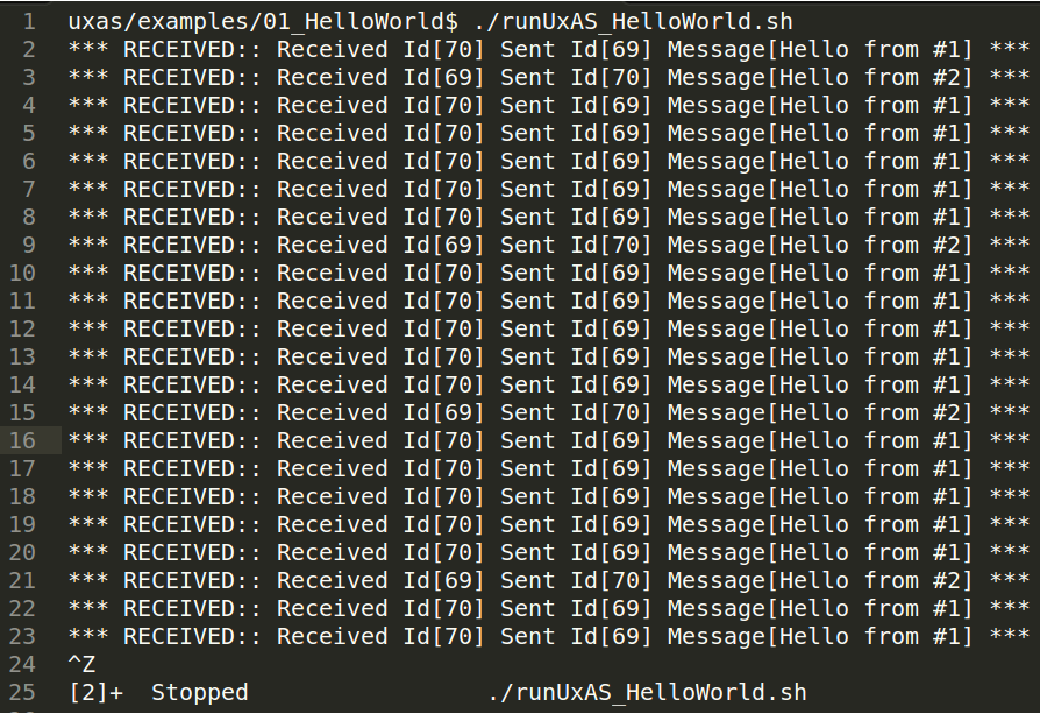
\includegraphics[width=1.3\linewidth]{\FiguresPath//01_ScreenCapture}
	\caption{HelloWorld console messages.}
	\label{fig:HelloWorldConsole}
\end{marginfigure}

\subsection{Coding the Hello World Example}
The two files:
\begin{docspec}
    uxas/code/src/Services/01\_HelloWorld.cpp
\end{docspec}
\begin{docspec}
    uxas/code/src/Services/01\_HelloWorld.h
\end{docspec}
contain the source code for the \textbf{\textit{HelloWorld}} service. These files were constructed using copies of the service template files:
\begin{docspec}
    uxas/code/src/Services/00\_ServiceTemplate.cpp
\end{docspec}
\begin{docspec}
    uxas/code/src/Services/00\_ServiceTemplate.h
\end{docspec}
Significant Modifications to the file \textit{00\_ServiceTemplate.h} consisted of:
\begin{description}
\item[a callback function for the timer]:\begin{docspec}void OnSendMessage();\end{docspec}
\item[a string to store messages to send]:\begin{docspec}std::string m\_stringToSend = std::string("Hello World!");\end{docspec}
\item[an int64 to store the send period]:\begin{docspec}int64\_t m\_sendPeriod\_ms\{1000\};\end{docspec}
\item[a uint64 to store the ID of the timer]:\begin{docspec}uint64\_t m\_sendMessageTimerId\{0\}; \end{docspec}
\end{description}

The \textbf{\textit{HelloWorld}} service was implemented by:
\begin{enumerate}
\item Handling the parameters \textit{StringToSend} and \textit{SendPeriod\_ms} in the \textit{HelloWorld::configure} virtual method.
\item Instantiating a \textit{uxas::common::TimerManager} timer in the \textit{HelloWorld::initialize()} virtual method.
\item Starting the timer in the \textit{HelloWorld::start()} virtual method.
\item Destroying the timer in the \textit{HelloWorld::terminate()} virtual method.
\item Printing out the string for any received messages in the \textit{HelloWorld::processReceivedLmcpMessage} virtual method.
\item Sending the message when timer times out in the \textit{HelloWorld::OnSendMessage()} method.
\end{enumerate}




\subsection{Hello World Example - Specifics}

This is a basic example of a UxAS service that sends/receives \textit{KeyValuePair} messages and prints out the results. 

\newthought{Files}
\begin{description}
\item[runUxAS\_HelloWorld.sh] - This is a bash shell script used to execute the example

\item[cfg\_HelloWorld.xml] - This is the file used to configure the example for UxAS

\item[01\_HelloWorld.cpp] - the C++ source code for the example. Note: this file is located in the following directory:
        code/src/Services/

\item[01\_HelloWorld.h] - the C++ header file for the example. Note: this file is located in the following directory:
        code/src/Services/
\end{description}

\newthought{Running the Example}
\begin{enumerate}
\item open a ternimal window in the directory: "examples/01\_HelloWorld/"
\item enter the command: `./runUxAS\_HelloWorld.sh`
\end{enumerate}

\newthought{What Happens?}
\begin{itemize}
\item Two copies of the HelloWorld service start up and begin sending messages. One copy sends a message once a second and the other sends a message every 5 seconds. Each service receives the messsages sent by the other service. When messages are received the services print them out.
\end{itemize} 

\newthought{Things to Try}
\begin{itemize}
\item Change the rate that messages are sent out. This is done by editing the `cfg\_HelloWorld.xml` file and changing the value of `SendPeriod\_ms`. Note: the time is entered in milliseconds, i.e. 1000 milliseconds == 1 second.
\item Change the message sent by each of the services. This is done by editing the `cfg\_HelloWorld.xml` file and changing the value of `StringToSend`.
\end{itemize} 



